%\documentclass{article}
%\usepackage{tikzpeople}
%\usepackage{tikz}
%\usepackage{graphicx}
%\usetikzlibrary{shapes, shapes.misc}
%\usetikzlibrary{arrows, arrows.meta, decorations.markings}
%\usetikzlibrary{patterns}
%\usetikzlibrary{positioning}


\makeatletter
% copied from the manual
\pgfdeclareshape{document}{%
    \inheritsavedanchors[from=rectangle] % this is nearly a rectangle
    \inheritanchorborder[from=rectangle]
    \inheritanchor[from=rectangle]{center}
    \inheritanchor[from=rectangle]{north}
    \inheritanchor[from=rectangle]{south}
    \inheritanchor[from=rectangle]{west}
    \inheritanchor[from=rectangle]{east}
	\inheritanchor[from=rectangle]{south west}
	\inheritanchor[from=rectangle]{north west}
	\inheritanchor[from=rectangle]{south east}
	\inheritanchor[from=rectangle]{north east}
    % ... and possibly more
    \backgroundpath{% this is new
        % store lower right in xa/ya and upper right in xb/yb
        \southwest \pgf@xa=\pgf@x \pgf@ya=\pgf@y
        \northeast \pgf@xb=\pgf@x \pgf@yb=\pgf@y
        \def\hangout{5pt}
        % compute corner of "flipped page"
        \pgf@xc=\pgf@xb \advance\pgf@xc by-\hangout % this should be a parameter
        \pgf@yc=\pgf@yb \advance\pgf@yc by-\hangout
        % construct main path
        \pgfpathmoveto{\pgfpoint{\pgf@xa}{\pgf@ya}}
        \pgfpathlineto{\pgfpoint{\pgf@xa}{\pgf@yb}}
        \pgfpathlineto{\pgfpoint{\pgf@xc}{\pgf@yb}}
        \pgfpathlineto{\pgfpoint{\pgf@xb}{\pgf@yc}}
        \pgfpathlineto{\pgfpoint{\pgf@xb}{\pgf@ya}}
        \pgfpathclose
        % add little corner
        \pgfpathmoveto{\pgfpoint{\pgf@xc}{\pgf@yb}}
        \pgfpathlineto{\pgfpoint{\pgf@xc}{\pgf@yc}}
        \pgfpathlineto{\pgfpoint{\pgf@xb}{\pgf@yc}}
        \pgfpathlineto{\pgfpoint{\pgf@xc}{\pgf@yc}}
        \pgfpathclose
        % add lines
        %\pgfmathsetmacro{\step}{round(abs(\pgf@yb-\pgf@ya)/6)}
        %\pgfmathsetmacro{\lines}{round(abs(\pgf@yb-\pgf@ya)/\step)-1}
        %\foreach \y in {1,...,\lines}{%
        %    \pgfpathmoveto{\pgfpoint{\pgf@xa+\step*1pt+\hangout}{\pgf@yb-\y*\step*1pt}}
        %    \pgfpathlineto{\pgfpoint{\pgf@xc-\step*1pt}{\pgf@yb-\y*\step*1pt}}
        %}%  
    }%
}%
\makeatother

%\begin{document}
\begin{center}
\resizebox{\columnwidth}{!}{%
\begin{tikzpicture}[>=latex]
\tikzstyle{every node}=[font=\Large]
\tikzstyle{apps} = [draw, very thick, minimum height=30pt, minimum width=50pt, fill=white, rectangle, font={\sffamily\bfseries}]
\tikzstyle{systemComp} = [draw, very thick, minimum height=30pt, minimum width=150pt, pattern= north west lines, pattern color = black!20!, rectangle, font={\sffamily\bfseries}]
\tikzstyle{doc} = [draw, thick, shape=document, align=left, color=black, minimum width=150pt, minimum height=40pt, inner sep=2ex]
\tikzstyle{vecarrow} = [->, thick, line width=5pt]
\tikzstyle{gthread} = [label={[font=\normalsize, red]below:#1}]
\tikzstyle{gnode} = [draw, thick, font=\normalsize, align =left, minimum width=18pt, minimum height=36pt]

\tikzset{ext/.pic={
\path [fill=white] (-0.2,0)to[bend left](0,0.1)to[bend right](0.2,0.2)to(0.2,0)to[bend left](0,-0.1)to[bend right](-0.2,-0.2)--cycle;
\draw (-0.2,0)to[bend left](0,0.1)to[bend right](0.2,0.2) (0.2,0)to[bend left](0,-0.1)to[bend right](-0.2,-0.2);
}}

%%draw MacOS components
\node [apps, name = software1] at (0, 0) {
\includegraphics[width=20pt]{./chromium_logo.png}};
\node [apps, name = software2, right of=software1, node distance=50pt] {daemon1};
\node [apps, name = software3, right of=software2, node distance=50pt] {daemon2};
\node [systemComp, name = libs, below of = software2, node distance =30pt] {Argus Instrumented Libraries};
\node [systemComp, name = os, below of = libs, node distance =30pt] {Argus Instrumented OS};

%% draw Tracing Event log
\node (TracingEventLog) [minimum height=30pt, minimum width=200pt, right of=software3, node distance=220pt]{};
\node (log) [doc, below of=TracingEventLog, node distance=30pt] {\#timestamp, event\_type, attr1, attr2...\\30.4, sendMessge, tid1, tid2 ..\\31.7, wakeUp, tid0, tid2...\\33.2, wakeUp, tid2, tid3...\\34.2, sendMessage, tid3, tid2...\\34.9, wakeUp, tid2, tid0...\\ ... ... };
\draw [vecarrow] (libs.east)+(0.5, 0) -- (log.west);

%draw Interactive Debugger 
\node (InteractiveDebugger) [systemComp, rounded corners=20pt, minimum height=280pt, minimum width=300pt, below left = 20pt and -160pt of log] {};
\node (debugger)[minimum width=220pt, above = -30pt of InteractiveDebugger]{Interactive Debugger};
\node (graph) [minimum height = 220pt, minimum width = 220pt, below = 10pt of debugger] {};
\node (shape) [doc, minimum height = 220pt, minimum width = 220pt, below = 10pt of debugger]{};

%\node [minimum width = 100pt, above = -20pt of graph, label=right:{graph}]{};
\node(ts)[gthread = browser, minimum width = 2pt, below left = -220pt and -40pt of graph, font=\scriptsize]{tid\_block};
\node(te)[gthread = browser, minimum width = 2pt, below left = -20pt and -34pt of graph]{};
\node(t0s)[gthread = browser, minimum width = 2pt, below left = -220pt and -75pt of graph, font=\scriptsize]{tid0};
\node(t0e)[gthread = browser, minimum width = 2pt, below left = -20pt and -69pt of graph]{};
\node(t1s)[gthread = kern, minimum width = 2pt, below left = -220pt and -105pt of graph, font=\scriptsize]{tid1};
\node(t1e)[gthread = kern, minimum width = 2pt, below left = -20pt and -99pt of graph]{};
\node(t2s)[gthread = renderer, minimum width = 2pt, below left = -220pt and -140pt of graph, font=\scriptsize]{tid2};
\node(t2e)[gthread = renderer, minimum width = 2pt, below left = -20pt and -134pt of graph]{};
\node(t3s)[gthread = renderer, minimum width = 2pt, below left = -220pt and -175pt of graph, font=\scriptsize]{tid3};
\node(t3e)[gthread = renderer, minimum width = 2pt, below left = -20pt and -169pt of graph]{};
\node(t4s)[gthread = fontd, minimum width = 2pt, below left = -220pt and -205pt of graph, font=\scriptsize]{tid4};
\node(t4e)[gthread = fontd, minimum width = 2pt, below left = -20pt and -199pt of graph]{};

\node(brw) [gnode, below = 80pt of ts, align=center, label={[font=\small]above:{similar node}}]{msg\\cv\_wait};
\node(brwb) [gnode, fill = black!20, below = 40pt of brw, align=center, label={[font=\small]above:{blocking node}}]{msg\\cv\_wait};
\node(brw0) [gnode, fill = blue!20, below = 20pt of t0s]{msg\\msg};
\node(brw1) [gnode, below = 15pt of brw0]{write\\msg};
\node(brw2) [gnode, below = 20pt of brw1]{read\\wake};
\node(k0) [gnode, fill = red!20, below = 25pt of t1s] {msg};
\node(k1) [gnode, below = 50pt of k0] {msg\\wait};
\node(rdw0) [gnode, fill = yellow!20, below = 30pt of t2s]{msg\\read\\msg};
\node(rdw1) [gnode, below = 30pt of rdw0]{msg\\msg};
\node(rdm0) [gnode, below = 40pt of t3s]{read\\msg};
\node(rdm1) [gnode, minimum height = 20pt, below = 20pt of rdm0]{write\\msg};
\node(rdm2) [gnode, thick, fill = black!20, minimum height = 10pt, below = 18pt of rdm1, font=\small]{msg\\sema\_wait};
\node(fontd0) [gnode, minimum height=20pt, below = 50pt of t4s]{msg\\msg};


\draw[-, solid](ts.south)--(brw);
\draw[-, solid](brw) -- pic{ext}(brwb);
\draw[-, dotted](brwb) --(ts.south);
\draw[-, solid](t0s.south) -- (brw0);
\draw[-, dotted](brw0) -- (brw1);
\draw[-, dotted](brw1) -- (brw2);
\draw[-, solid](brw2) -- (t0e.south);
\draw[-, solid](t1s.south) -- (k0);
\draw[-, dotted](k0) -- (k1);
\draw[-, dotted](k1) -- (t1e.south);
\draw[-, solid](t2s.south) -- (rdw0);
\draw[-, dotted](rdw0) -- (rdw1);
\draw[-, solid](rdw1) -- (t2e.south);
\draw[-, solid](t3s.south) -- (rdm0);
\draw[-, dotted](rdm0) -- (rdm1);
\draw[-, solid](rdm1) --pic{ext}(rdm2);
\draw[-, solid](t4s) -- (fontd0);
\draw[-, dotted](rdm2) -- (t3e.south);
\draw[-, solid](fontd0) --(t4e.south);


\draw[->, dotted, thick] (brw) -- (brw2);
\draw[->] (brw0.east) -- node[font=\small, minimum width=5pt, pos=0.1, below]{e0} (rdw0.west);
\draw[->] (k0.east) -- node[font=\small, minimum width=5pt, above]{e1} (rdw0.west);
\draw[->] (rdw0.east) -- (rdm0.west);
\draw[->] (rdm0.east) -- (fontd0.west);
\draw[->] (fontd0.south) -- (rdm1.east);
\draw[->] (rdm1.west) -- (rdw1.east);
\draw[->] (rdw1.west) -- (brw2.east);


\draw [vecarrow] (log.south) -- (InteractiveDebugger);

\node (legend)[minimum height =180pt, minimum width = 80pt, right of = InteractiveDebugger, node distance= 200pt]{};
\node (1)[below left = -20pt and -20pt of legend] {};
\node (2)[right=8pt of 1]{};
\draw [-, solid] (1.east) -- (2);
\node [right= 10pt of 1, font=\large]{thread\_running};

\node (3)[below left = -30pt and -20pt of legend] {};
\node (4)[right=8pt of 3]{};
\draw [-, dotted] (3.east) -- (4);
\node [right =10pt of 3, font=\large]{thread\_wait};

\node (5)[below left = -40pt and -20pt of legend] {};
\node (6)[right =8pt of 5]{};
\draw [->] (5.east) -- (6);
\node [right =10pt of 5, font=\large]{edge};

\node (7)[below left = -50pt and -20pt of legend] {};
\node (8)[right =8pt of 7]{};
\draw [->, dotted, thick] (7.east) -- (8);
\node [right =10pt of 7, font=\large]{weak edge};

\node [draw, solid, minimum width = 10pt, minimum height = 3pt, below left = -60pt and -30pt of legend, label={[font=\large]right:node}]{};

%draw interactive Debugging part
\umlactor[left = 100pt of InteractiveDebugger, scale=2]{user};
\node (user)[left = 100pt of InteractiveDebugger]{};
%\node (query1)[above left = -80pt and -10pt of InteractiveDebugger]{};
%\node (query2)[above left = -100pt and -10pt of InteractiveDebugger]{};
\node (query3)[below left = -100pt and -10pt of InteractiveDebugger]{};
\node (query4)[below left = -80pt and -10pt of InteractiveDebugger]{};
%\draw [->, thick, out=160, in=60] (query1.north west) to node{which node?} (user.north);
%\draw [->, thick, out=350, in=230] (user.north) to node{node 5} (query2.north west);
\draw [->, thick, out=150, in=30] (query3.north west) to node {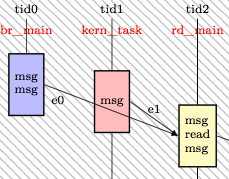
\includegraphics[width=60pt]{./graph_snippet.png}} (user.south);
\draw [->, thick, out=310, in=230] (user.south) to node[above]{e0} (query4.north);

\node (result) [draw, dotted, minimum height = 100pt, minimum width = 400pt,pattern= north west lines, pattern color = black!30, below = 30pt of InteractiveDebugger]{};
\node (blockrenderer) [draw, solid, minimum height = 10pt, fill=black!20, below left = -40pt and -200pt of result, label=below:render thread blocks on semaphore]{msg sema\_wait};
\node (blockbrowser) [draw, solid, minimum height = 10pt, fill=black!20, below left = -80pt and -200pt of result, label=above:browser thread blocks on condition variable]{msg cv\_wait};

\draw[->, out=330, in = 45](blockrenderer.east)  -- pic{ext} (blockbrowser.east);
\draw[->, out=230, in = 135](blockbrowser.west) -- pic{ext} (blockrenderer.west);
%\node (text1)[below = 50pt of = blockrenderer] {renderer thread \\blocks on semaphore};
%\node (text1)[below = 50pt of = blockbrowser] {browser thread \\blocks on conditional variable};

\draw [vecarrow] (InteractiveDebugger.south) -- (result);
\end{tikzpicture}
}
\end{center}
%\end{document}
